\documentclass[11pt,psfig]{article}
\usepackage{epsfig}
\usepackage{times}
\usepackage{amssymb}
\usepackage{float}

\newcount\refno\refno=1
\def\ref{\the\refno \global\advance\refno by 1}
\def\ux{\underline{x}}
\def\uw{\underline{w}}
\def\bw{\underline{w}}
\def\ut{\underline{\theta}}
\def\umu{\underline{\mu}} 
\def\bmu{\underline{\mu}} 
\def\be{p_e^*}
\newcount\eqnumber\eqnumber=1
\def\eq{\the \eqnumber \global\advance\eqnumber by 1}
\def\eqs{\eq}
\def\eqn{\eqno(\eq)}

 \pagestyle{empty}
\def\baselinestretch{1.1}
\topmargin1in \headsep0.3in
\topmargin0in \oddsidemargin0in \textwidth6.5in \textheight8.5in
\begin{document}
\setlength{\parskip}{1.2ex plus0.3ex minus 0.3ex}


\thispagestyle{empty} \pagestyle{myheadings} \markright{Homework
4: CS 216, Image Understanding: Spring 2014}



\title{CS 216 Homework 4}
\author{Zachary DeStefano, 15247592}
\date{Due Date: May 23, 2014}

\maketitle

\vfill\eject

\newpage

\section*{Single Scale Detector Output}

\subsection*{Output for test1.jpg}

\begin{figure}[H]
\centering
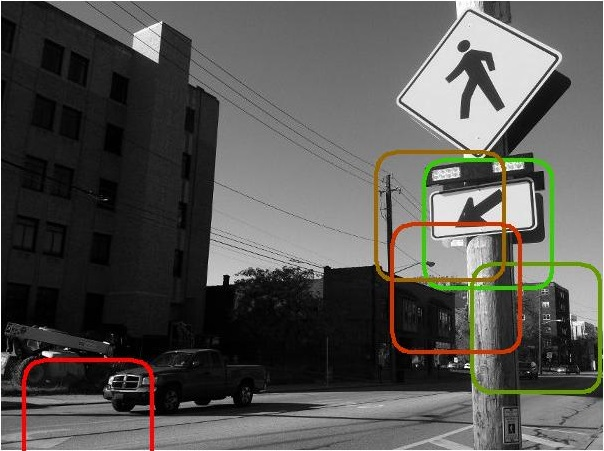
\includegraphics[height=3in]{prob5_a1plot1.jpg}
\caption{Detector Output with single positive template}
\end{figure}

\begin{figure}[H]
\centering
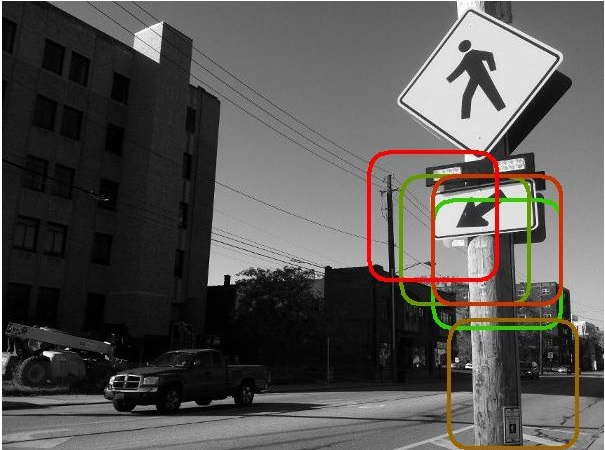
\includegraphics[height=3in]{prob5_a2plot1.jpg}
\caption{Detector Output with 5 positive templates}
\end{figure}

\begin{figure}[H]
\centering
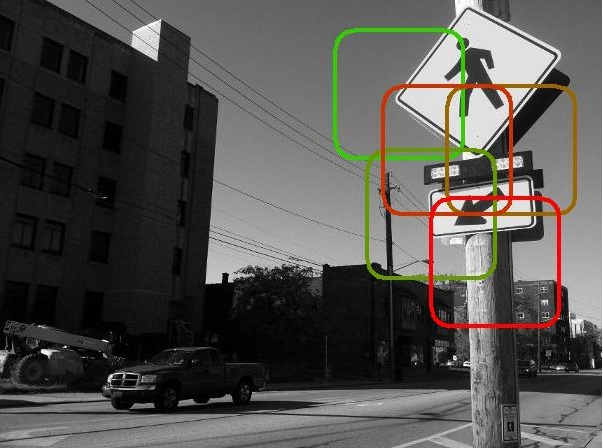
\includegraphics[height=3in]{prob5_a3plot1.jpg}
\caption{Detector Output with 5 positive templates and 100 negative templates}
\end{figure}

\subsection*{Output for test4.jpg}

\begin{figure}[H]
\centering
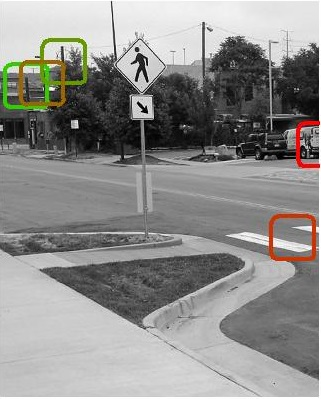
\includegraphics[height=3in]{prob5_a1plot2.jpg}
\caption{Detector Output with single positive template}
\end{figure}

\begin{figure}[H]
\centering
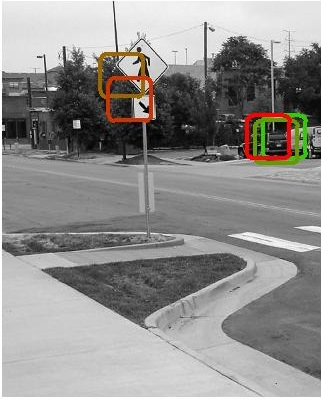
\includegraphics[height=3in]{prob5_a2plot2.jpg}
\caption{Detector Output with 5 positive templates}
\end{figure}

\begin{figure}[H]
\centering
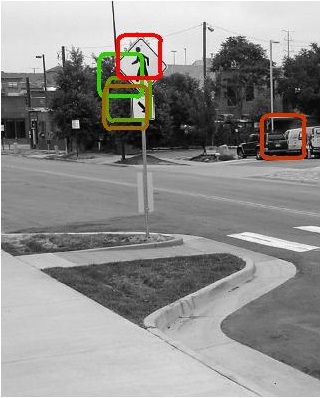
\includegraphics[height=3in]{prob5_a3plot2.jpg}
\caption{Detector Output with 5 positive templates and 100 negative templates}
\end{figure}

\section*{Multiscale Detector Output}

\subsection*{Final Output for test images}

I used 0.7 as a scale factor. The best results ended up being at the first level in the image pyramid, so in the next section are the detected results at each of the other levels of the pyramid. 

\begin{figure}[H]
\centering
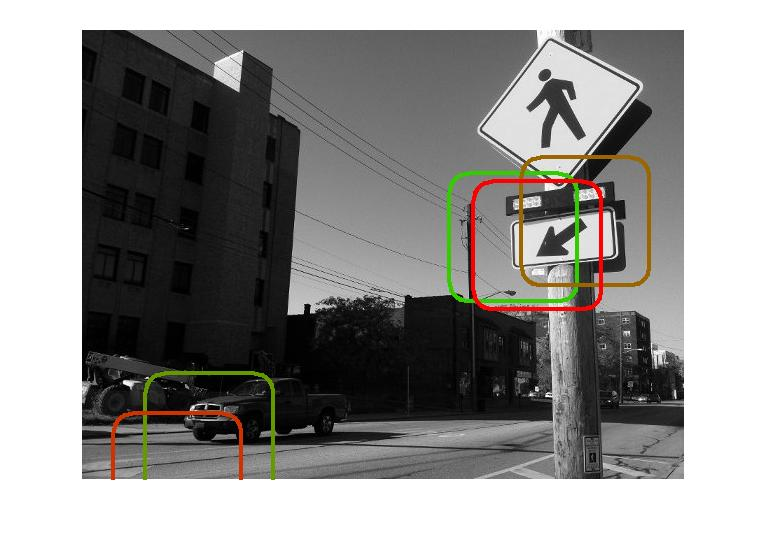
\includegraphics[height=3in]{prob5b_plot1.jpg}
\caption{Final multi scale detector output for test1.jpg}
\end{figure}

\begin{figure}[H]
\centering
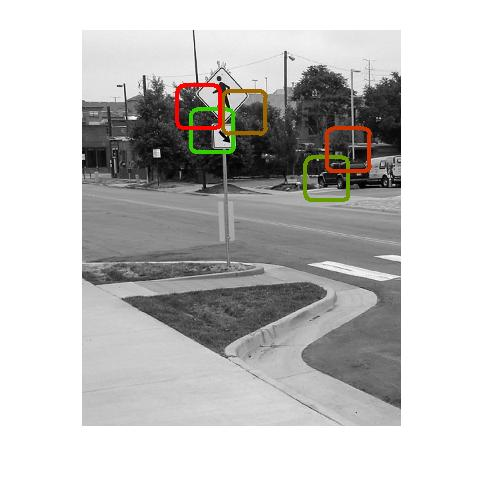
\includegraphics[height=3in]{prob5b_plot2.jpg}
\caption{Final multi scale detector output for test4.jpg}
\end{figure}

\subsection*{Output at multiple scales for test1.jpg}

\begin{figure}[H]
\centering
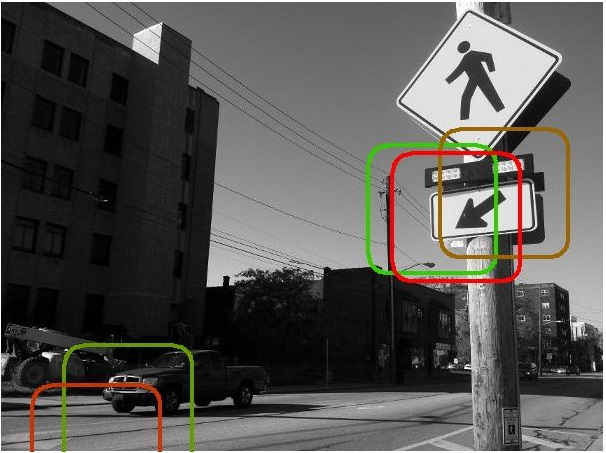
\includegraphics[height=4in]{prob5b_plot1_level1.jpg}
\caption{Detector output for test1.jpg at level 1 in image pyramid}
\end{figure}

\begin{figure}[H]
\centering
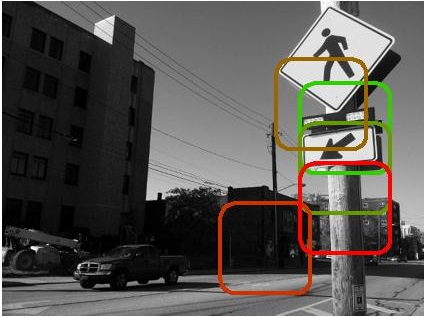
\includegraphics[height=3in]{prob5b_plot1_level2.jpg}
\caption{Detector output for test1.jpg at level 2 in image pyramid}
\end{figure}

\begin{figure}[H]
\centering
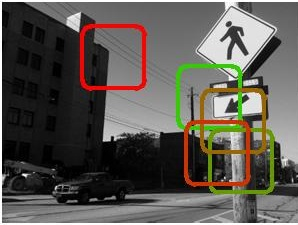
\includegraphics[height=2in]{prob5b_plot1_level3.jpg}
\caption{Detector output for test1.jpg at level 3 in image pyramid}
\end{figure}

\subsection*{Output at multiple scales for test4.jpg}

\begin{figure}[H]
\centering
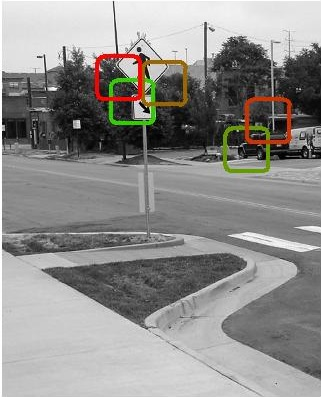
\includegraphics[height=4in]{prob5b_plot2_level1.jpg}
\caption{Detector output for test4.jpg at level 1 in image pyramid}
\end{figure}

\begin{figure}[H]
\centering
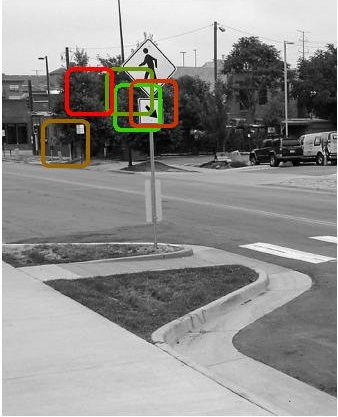
\includegraphics[height=3.5in]{prob5b_plot2_level2.jpg}
\caption{Detector output for test4.jpg at level 2 in image pyramid}
\end{figure}

\begin{figure}[H]
\centering
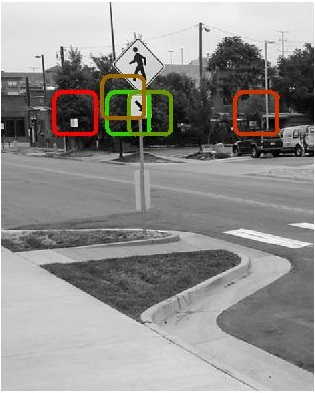
\includegraphics[height=3in]{prob5b_plot2_level3.jpg}
\caption{Detector output for test4.jpg at level 3 in image pyramid}
\end{figure}

\begin{figure}[H]
\centering
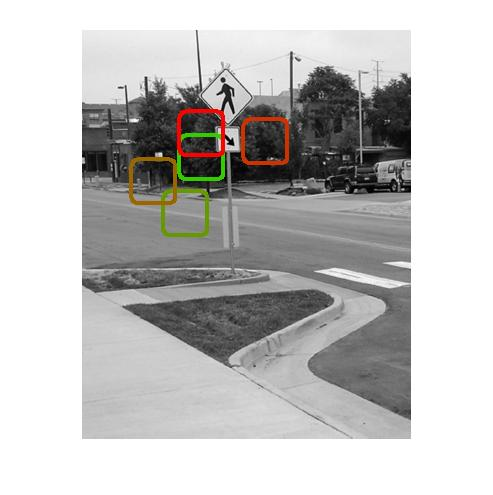
\includegraphics[height=2.5in]{prob5b_plot2_level4.jpg}
\caption{Detector output for test4.jpg at level 4 in image pyramid}
\end{figure}

\begin{figure}[H]
\centering
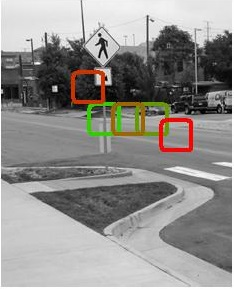
\includegraphics[height=2in]{prob5b_plot2_level5.jpg}
\caption{Detector output for test4.jpg at level 5 in image pyramid}
\end{figure}

\section*{Templates Used for Detection}

\subsection*{The Five Positive Templates}

\begin{figure}[H]
\centering
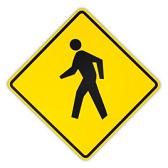
\includegraphics[height=2in]{prob4posTrain/pedSign2Train.jpg}
\caption{Pedestrian sign image from internet}
\end{figure}

\begin{figure}[H]
\centering
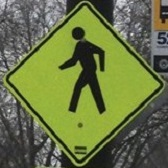
\includegraphics[height=2in]{prob4posTrain/test3train.jpg}
\caption{Pedestrian sign image from test3.jpg}
\end{figure}

\begin{figure}[H]
\centering
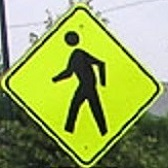
\includegraphics[height=2in]{prob4posTrain/test4train.jpg}
\caption{Pedestrian sign image from test4.jpg}
\end{figure}

\begin{figure}[H]
\centering
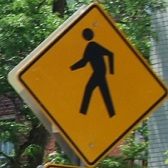
\includegraphics[height=2in]{prob4posTrain/test5train.jpg}
\caption{Pedestrian sign image from test5.jpg}
\end{figure}

\begin{figure}[H]
\centering
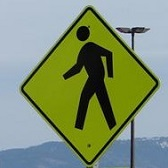
\includegraphics[height=2in]{prob4posTrain/test6train.jpg}
\caption{Pedestrian sign image from test6.jpg}
\end{figure}

\subsection*{The 100 negative examples}

These are in the zip file containing the code inside a folder entitled \"prob4negTrain\". 


\end{document}








